\begin{center}
	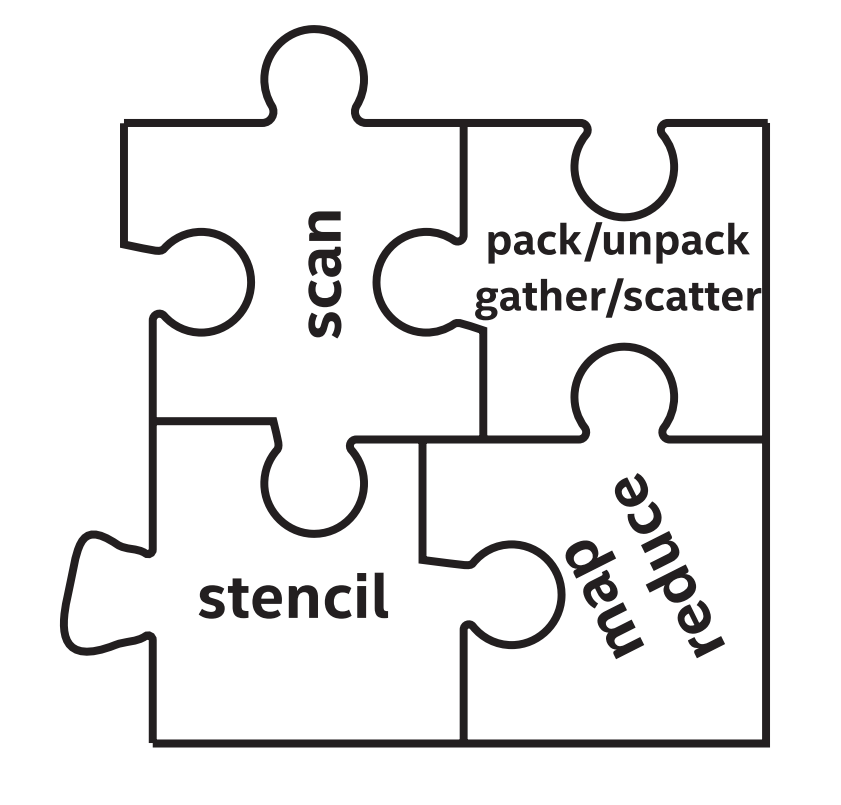
\includegraphics[width=0.5\textwidth]{content/chapter-14/images/1}
\end{center}

When we are at our best as programmers, we recognize patterns in our work and apply techniques that are time proven to be the best solution. Parallel programming is no different, and it would be a serious mistake not to study the patterns that have proven to be useful in this space. Consider the MapReduce frameworks adopted for Big Data applications; their success stems largely from being based on two simple yet effective parallel patterns—map and reduce.\par

There are a number of common patterns in parallel programming that crop up time and again, independent of the programming language that we’re using. These patterns are versatile and can be employed at any level of parallelism (e.g., sub-groups, work-groups, full devices) and on any device (e.g., CPUs, GPUs, FPGAs). However, certain properties of the patterns (such as their scalability) may affect their suitability for different devices. In some cases, adapting an application to a new device may simply require choosing appropriate parameters or fine-tuning an implementation of a pattern; in others, we may be able to improve performance by selecting a different pattern entirely.\par

Developing an understanding of how, when, and where to use these common parallel patterns is a key part of improving our proficiency in DPC++ (and parallel programming in general). For those with existing parallel programming experience, seeing how these patterns are expressed in DPC++ can be a quick way to spin up and gain familiarity with the capabilities of the language.\par

This chapter aims to provide answers to the following questions:\par

\begin{itemize}
	\item Which patterns are the most important to understand?
	\item How do the patterns relate to the capabilities of different devices?
	\item Which patterns are already provided as DPC++ functions and libraries?
	\item How would the patterns be implemented using direct programming?
\end{itemize}










